\documentclass{beamer}
\title{JWT Authentication and Authorization}
\author{Ilya Averyanov}
\institute{EMQX}
\date{2022}
\usetheme{emqx}
\usepackage{listings}
\usepackage{color}
\usepackage{graphicx}
\usepackage{xcolor}
\usepackage{hyperref}
\definecolor{href}{rgb}{0,0,0.9375}
\hypersetup{
    pdfborderstyle={/S/U/W 1}, % underline links instead of boxes
    colorlinks=true,
    urlcolor=href
}
\lstset{frame=tb,
  aboveskip=3mm,
  belowskip=3mm,
  showstringspaces=false,
  columns=flexible,
  basicstyle={\small\ttfamily},
  numbers=none,
  numberstyle=\tiny\color{gray},
  keywordstyle=\color{blue},
  commentstyle=\color{dkgreen},
  stringstyle=\color{mauve},
  breaklines=true,
  breakatwhitespace=false,
  tabsize=2
}


\begin{document}

\frame{\titlepage}

% \begin{frame}
%     \frametitle{feature}
%     \framesubtitle{Externally}

%     \begin{itemize}
%         \item Each topic can have a \textit{retained} message
%         \item This message is sent to each subscriber on topic subscribe
%         \item A subscriber can subscribe to many topics at once using wildcards and receive many
%         retained messages
%     \end{itemize}

%     \begin{center}
%         \includegraphics[width=10cm, keepaspectratio]{images/retain-demo.png}
%     \end{center}
%     \lstinline{DeviceModel} and \lstinline{Owner}.

%     \vspace{1cm}

%     \begin{lstlisting}
%       lst
%     \end{lstlisting}

% \end{frame}

\begin{frame}
    \frametitle{JWT}
    \framesubtitle{JSON Web Token}

    \textbf{JSON Web Token} (\textbf{JWT}) is a compact, URL-safe means of representing
    claims to be transferred between two parties. The \textbf{claims} in a JWT
    are encoded as a \textbf{JSON object} that is used as the payload of a JSON
    Web Signature (JWS) structure or as the plaintext of a JSON Web
    Encryption (JWE) structure, enabling the claims to be digitally
    signed or integrity protected with a Message Authentication Code
    (MAC) and/or encrypted.
\end{frame}

\begin{frame}
    \frametitle{JWT}
    \framesubtitle{JSON Web Token}

    \begin{itemize}
        \item \href{https://datatracker.ietf.org/doc/html/rfc7519}{https://datatracker.ietf.org/doc/html/rfc7519}.
        \item \textit{Claims} are actually predefined or custom fields.
        \item Generally, JSON Web Signature (JWS) structure is implied for JWTs.
    \end{itemize}
\end{frame}

\begin{frame}
    \frametitle{JWT}
    \framesubtitle{JWT Structure}

    \begin{itemize}
        \item Base64 encoded JSON header with signature algorithm and other signature params.
        \item Base64 encoded JSON payload with claims.
        \item Base64 signature of header and payload.
    \end{itemize}
    The parts are conactenated with the period
\end{frame}


\begin{frame}
    \frametitle{JWT}
    \framesubtitle{JWT Structure}

    \begin{center}
        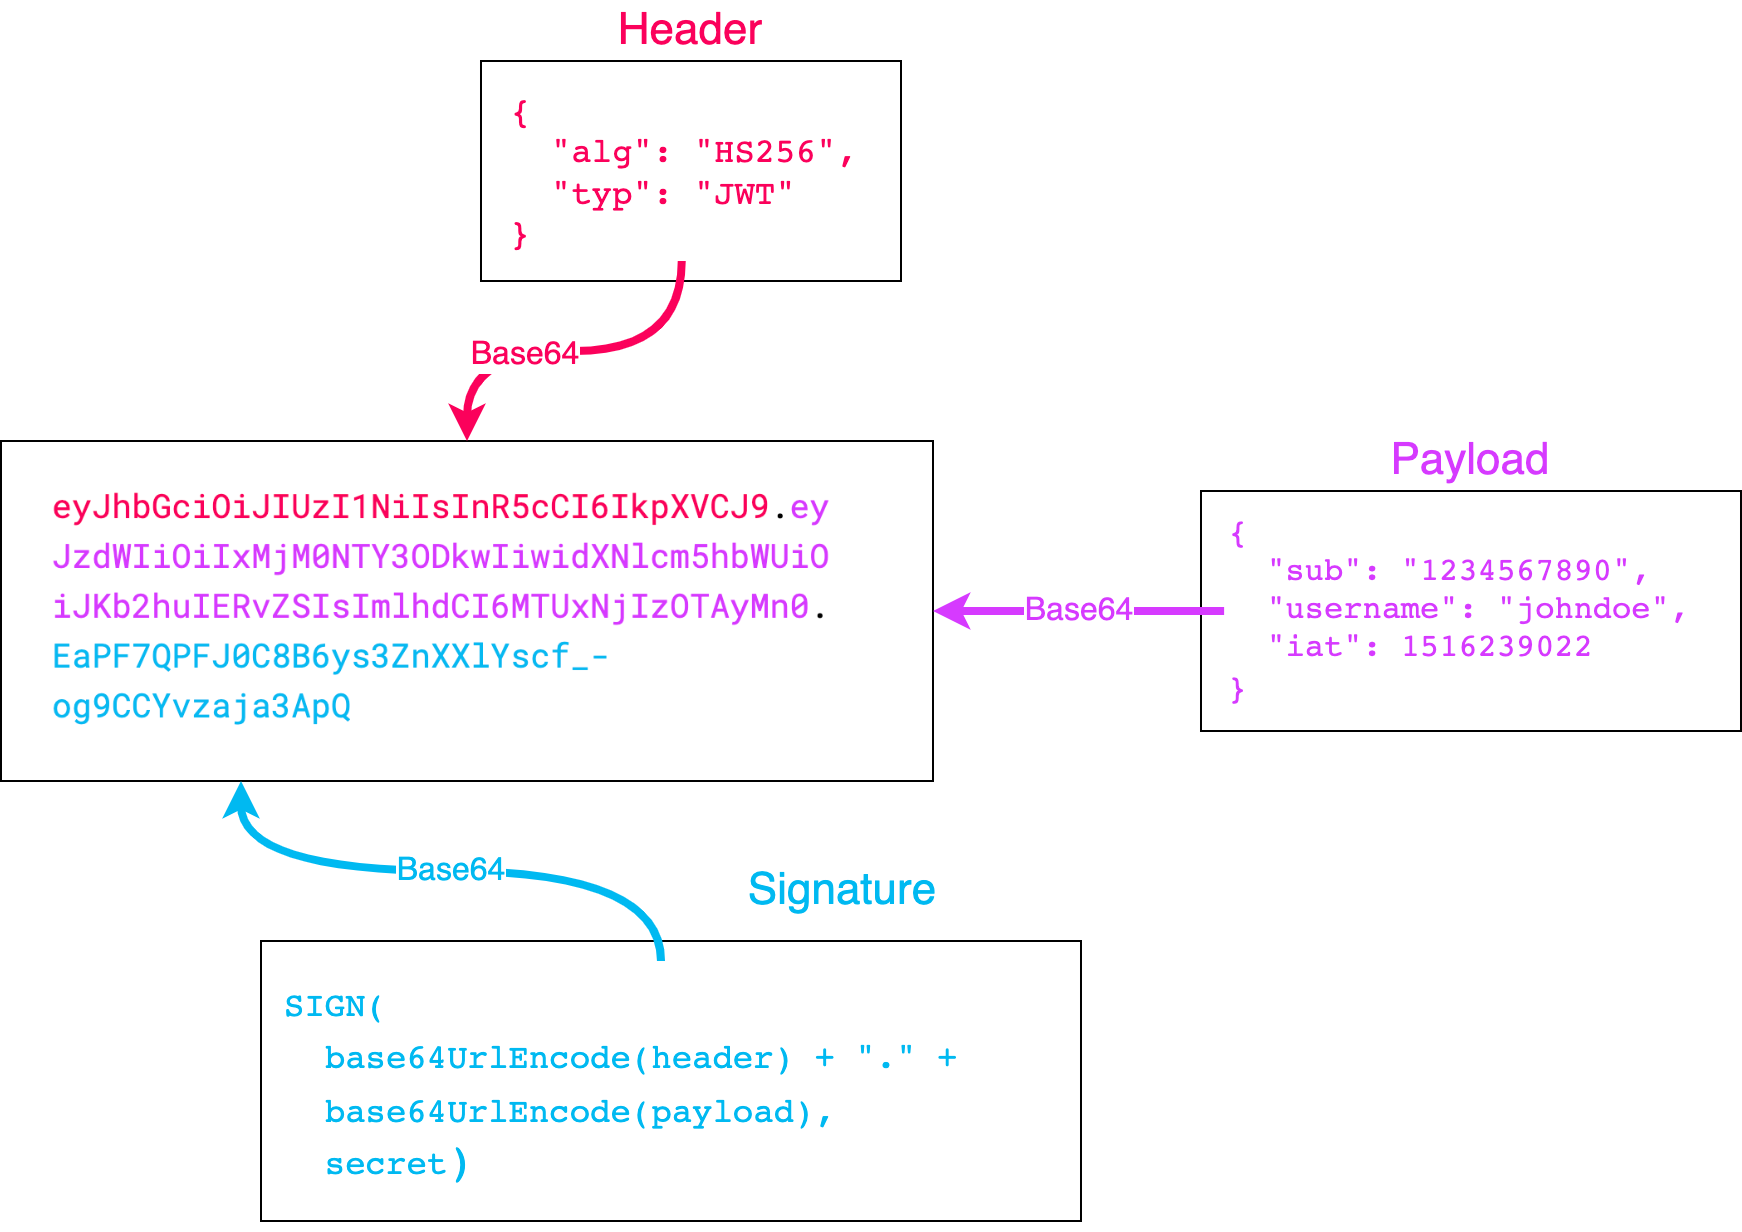
\includegraphics[width=8cm, keepaspectratio]{images/jwt-structure.png}
    \end{center}
\end{frame}

\begin{frame}
    \frametitle{JWT Authentication}
    \framesubtitle{EMQX}

    \begin{itemize}
        \item A client submits its credentials to an authentication server and exchanges them to a JWT.
        \item Connects to EMQX carrying JWT as username or password.
        \item EMQX verifies the signature and, optionally, JWT claims. If the checks pass, the authentication succeeds.
    \end{itemize}
\end{frame}

\begin{frame}
    \frametitle{JWT Authentication}
    \framesubtitle{EMQX}

    \begin{center}
        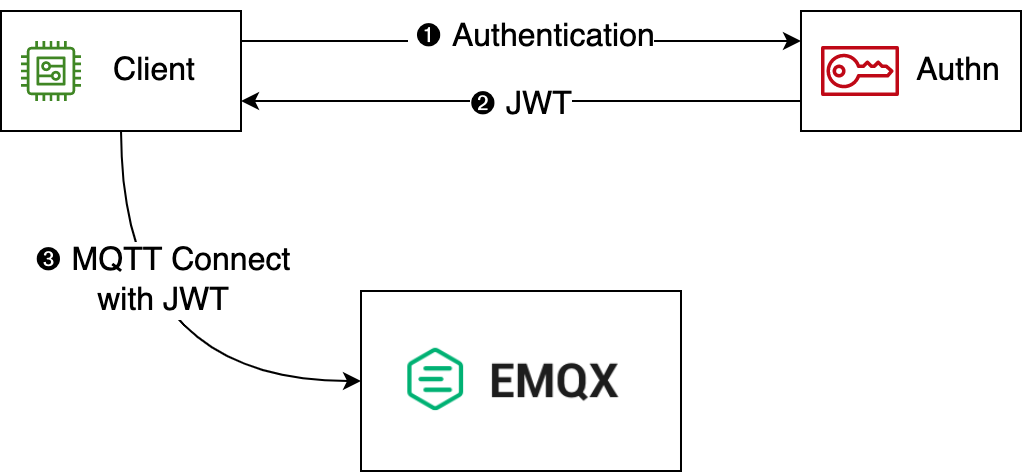
\includegraphics[width=8cm, keepaspectratio]{images/jwt-authn.png}
    \end{center}
\end{frame}

\begin{frame}
    \frametitle{JWT Authentication}
    \framesubtitle{Advantages}

    \begin{itemize}
        \item JWTs are a standard for service communication, there are many production-ready authentication servers supporting JWT exchange.
        \item JWTs are small and self-contained, so they are easy to manipulate.
        \item Authentication with JWT decouples credential management from EMQX. Users may choose their own mechanisms of provisioning clients with JWTs.
        \item Accessing EMQX with JWTs is lightweight. EMQX does not have to access any external resources to verify a JWT.
    \end{itemize}
\end{frame}

\begin{frame}
    \frametitle{JWT Authentication}
    \framesubtitle{Caveats}

    \begin{itemize}
        \item JWTs are signed, not encrypted. They should not contain sensitive information.
        \item JWTs cannot be revoked easily. So if stolen, JWTs can be used by an intruder until expiration. Therefore, JWT lifetimes should be chosen wisely.
        \item Use of SSL connection is strongly recommended to avoid JWT compromisation.
        \item If HMAC signatures are used, the secret must be stored securely by the accessed service (EMQX).
    \end{itemize}
\end{frame}

\begin{frame}[fragile]
    \frametitle{JWT Authentication}
    \framesubtitle{Enabling in EMQX}

    Enable \lstinline{emqx_auth_jwt} plugin in \lstinline{data/loaded_plugins}:
    \begin{lstlisting}
    ...
    {emqx_auth_jwt, true}.
    \end{lstlisting}
    Configure \lstinline{emqx_auth_jwt} in \lstinline{etc/plugins/emqx_auth_jwt.conf}:
    \begin{lstlisting}
    auth.jwt.secret = emqxsecret
    #auth.jwt.pubkey = etc/certs/jwt_public_key.pem
    #auth.jwt.jwks = https://auth.server/keys.json

    auth.jwt.from = password
    \end{lstlisting}
\end{frame}

\begin{frame}[fragile]
    \frametitle{JWT Authentication}
    \framesubtitle{Identity Verification}

    Authentication server issues JWTs with username or clientid claims:
    \begin{lstlisting}
    {
        "exp": 1656425413,
        "iat": 1656424813,
        "username": "someuser"
    }
    \end{lstlisting}
    Configure \lstinline{emqx_auth_jwt} to verify claims:
    \begin{lstlisting}
    ...
    auth.jwt.verify_claims = on
    auth.jwt.verify_claims.username = %u
    \end{lstlisting}
\end{frame}

\begin{frame}[fragile]
    \frametitle{JWT Authorization}
    \framesubtitle{ACL rules}

    Additionally, the authentication provides \lstinline{acl} claim with topic patterns
    available for publish(\lstinline{pub}), subscribe(\lstinline{sub}), and publish-subscribe(\lstinline{all}) operations:
    \begin{lstlisting}
    {
        ...
        "username": "someuser",
        "acl": {
            "sub": ["foo/#"],
            "pub": ["bar/#", "baz/#"]
        }
    }
    \end{lstlisting}
\end{frame}

\begin{frame}
    \begin{center}
        Thank you!
    \end{center}
\end{frame}

\end{document}
